\chapter{Parallelism: Multicore, Coherence, and Synchronisation}\label{ch:parallel}
\begin{center}\small\textit{Many cores, one memory: how to share correctly and quickly.}\end{center}

\section{From One Core to Many: Why Multicore?}
Frequency scaling hit a power wall: $P \propto CV^2 f$ and Pollack's rule says
single-core performance grows as $\sqrt{\text{area}}$---doubling area gives only
$\sim$40\% more speed. The industry answer was to duplicate cores: a chip-multiprocessor
(CMP) reuses the same core design $N$ times and lets software exploit thread-level
parallelism (TLP). Throughput then scales near-linearly if work parallelises, at the
cost of making shared memory correct.

Shared memory is intuitive: all cores see one address space, communication via
loads/stores. The hardware must make this illusion efficient while preserving
correctness. Two pillars do that: \textbf{cache coherence} (one value per address) and
\textbf{memory consistency} (order of values across addresses). Get them wrong and
programs see stale data or impossible reorderings.

\begin{definition}[Cache coherence vs.\ consistency]
\emph{Coherence} guarantees that writes to a single address become visible to all cores
in a total order (eventually every read sees the last write). \emph{Consistency} defines
the order in which writes to \emph{different} addresses become visible---the memory
model (SC, TSO, weak).
\end{definition}

Without coherence, core 0 could read $x=0$ from its cache while core 1 has just written
$x=1$ to its own cache---the system would violate the single-memory illusion. Every
private cache therefore participates in a coherence protocol.

\begin{center}
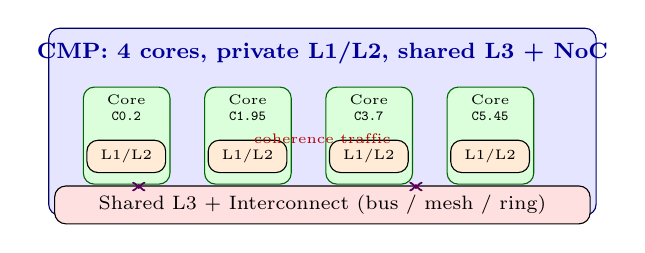
\begin{tikzpicture}[font=\scriptsize, scale=0.88]
\draw[fill=blue!10, draw=blue!40!black, rounded corners] (-0.3,-1.0) rectangle (7.6,1.7);
\node[font=\footnotesize\bfseries, text=blue!60!black] at (3.65,1.35) {CMP: 4 cores, private L1/L2, shared L3 + NoC};
\foreach \x in {0.2,1.95,3.7,5.45} {
  \draw[fill=green!14, draw=green!40!black, rounded corners] (\x,-0.55) rectangle (\x+1.25,0.85);
  \node[font=\tiny, align=center] at (\x+0.62,0.55) {Core\\\texttt{C\x}};
  \node[font=\tiny, fill=orange!16, draw, rounded corners, minimum width=1.0cm] at (\x+0.62,-0.15) {L1/L2};
}
\node[draw, fill=red!12, minimum width=6.8cm, minimum height=0.48cm, rounded corners] at (3.65,-0.85) {Shared L3 + Interconnect (bus / mesh / ring)};
\draw[<->, thick, violet!70!black] (1.0,-0.55) -- (1.0,-0.62);
\draw[<->, thick, violet!70!black] (5.0,-0.55) -- (5.0,-0.62);
\node[font=\tiny, text=red!70!black] at (3.65,0.10) {coherence traffic};
\end{tikzpicture}
\end{center}

\section{Cache Coherence: MSI and MESI}
The classic protocol is \textbf{MSI}: each block is Modified (dirty, exclusive), Shared
(clean, may be in many caches), or Invalid (not present). Stable states plus transient
states handle races. On a read miss, the cache issues \texttt{BusRd}; if another cache
holds M, it writes back and moves to S. On a write miss/hit to S, it issues
\texttt{BusRdX} (read-exclusive), invalidating all sharers.

MSI wastes traffic on first reads that will later be written (read then upgrade).
\textbf{MESI} adds Exclusive (clean, exclusive): a block loaded unshared enters E, and a
later write can silently upgrade E$\to$M without bus traffic. This common case (private
data) is why all real machines use MESI/MOESI/MESIF variants.

Two enforcement styles: \textbf{snooping} (all caches watch a bus/NoC broadcast, $O(N)$
broadcasts, simple, needs ordered interconnect) and \textbf{directory} (home node tracks
sharer list, point-to-point messages, scalable to many cores but indirection latency).
Modern chips snoop within a cluster and use directories between clusters.

\begin{center}
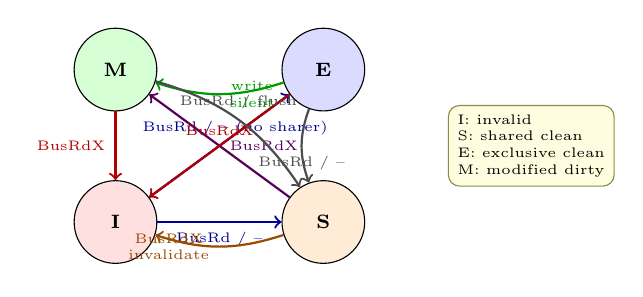
\begin{tikzpicture}[font=\scriptsize, scale=0.88, every node/.style={font=\scriptsize}]
\node[draw, fill=green!16, circle, minimum size=1.05cm] (m) at (0,1.2) {\textbf{M}};
\node[draw, fill=blue!14, circle, minimum size=1.05cm] (e) at (3.0,1.2) {\textbf{E}};
\node[draw, fill=orange!16, circle, minimum size=1.05cm] (s) at (3.0,-1.0) {\textbf{S}};
\node[draw, fill=red!12, circle, minimum size=1.05cm] (i) at (0,-1.0) {\textbf{I}};
\draw[->, thick, blue!60!black] (i) -- (s) node[midway, below, font=\tiny] {BusRd / --};
\draw[->, thick, blue!60!black] (i) -- (e) node[midway, above, font=\tiny, xshift=0.2cm] {BusRd / -- (no sharer)};
\draw[->, thick, green!60!black] (e) to[bend left=18] node[midway, right, font=\tiny, align=center] {write\\silent} (m);
\draw[->, thick, violet!70!black] (s) -- (m) node[midway, right, font=\tiny] {BusRdX};
\draw[->, thick, red!70!black] (m) -- (i) node[midway, left, font=\tiny] {BusRdX};
\draw[->, thick, red!70!black] (e) -- (i) node[midway, above, font=\tiny] {BusRdX};
\draw[->, thick, orange!60!black] (s) to[bend left=18] node[midway, left, font=\tiny, align=center] {BusRdX\\invalidate} (i);
\draw[->, thick, gray!60!black] (m) to[bend left=20] node[midway, above, font=\tiny] {BusRd / flush} (s);
\draw[->, thick, gray!60!black] (e) to[bend right=20] node[midway, below, font=\tiny] {BusRd / --} (s);
\node[font=\tiny, fill=yellow!12, draw=yellow!50!black, rounded corners, align=left] at (6.0,0.10) {I: invalid\\S: shared clean\\E: exclusive clean\\M: modified dirty};
\end{tikzpicture}
\end{center}

Coherence adds traffic and latency: a miss may need to invalidate $k$ sharers and wait
for acknowledgements. False sharing---two unrelated variables in the same 64\,B line
bouncing between cores---amplifies this. Padding or per-core batching fixes it.

\section{Consistency: What Order Do Writes Become Visible?}
Coherence says nothing about ordering across addresses. Consider Dekker's flag protocol:
core 0 does $x=1$; $r1=y$ and core 1 does $y=1$; $r2=x$. Under \textbf{sequential
consistency (SC)}---``all ops appear in one global order respecting each core's program
order''---$r1=r2=0$ is impossible (one write must precede the other's read). But modern
machines (x86 TSO, ARM weak) reorder to hide store latency with store buffers: both
reads can see 0, breaking Dekker.

x86 is TSO (total store order): loads bypass earlier stores to different addresses, but
stores are ordered and loads are ordered. ARM/RISC-V are weaker: almost any reordering
is allowed unless a \texttt{fence} is inserted. Compilers and programmers use
acquire/release annotations; hardware reorders freely underneath, gaining 10--30\%
performance while correctness is recovered by fences only where needed. The RISC-V
memory model even maps \texttt{acquire} to \texttt{fence r,rw}.

Understanding the memory model matters: 90\% of ``mysterious'' concurrency bugs are
missing fences or misunderstood atomics, not coherence. Tools like herd and litmus
tests let architects verify the model exhaustively.

\section{Directory Protocol and Scaling}
Snooping broadcasts to all cores---$O(N)$ messages per miss---which is untenable beyond
$\sim$32 cores. A \textbf{directory} stores, per block, the sharer bit-vector at the
home node. On a write, the writer contacts the directory, which point-to-point
invalidates only sharers. Cost is indirection (request $\to$ directory $\to$ sharers
$\to$ ack) and directory storage ($N$ bits per block). Sparse directories spill to
memory; coarse vectors trade false invalidations for smaller tags.

Modern hierarchies are hierarchical: snooping inside a 4--8 core cluster (low latency)
and directory between clusters/chiplets (scalable). AMD Zen and Intel Sapphire Rapids
use a mix---coherence is not one protocol but a family tuned to distance.

\section{Synchronisation and Atomic Primitives}
Cores synchronise with \textbf{atomic read-modify-write} ops: \texttt{test-and-set},
\texttt{fetch-and-add}, \texttt{compare-and-swap (CAS)}. Locks built from them need
care: a naive spinlock with \texttt{CAS} hammers the interconnect. Better:
\texttt{test-and-test-and-set} (spin on cached copy, CAS only when free) or queue locks
(MCS) where each waiter spins on its own line, eliminating invalidation storms.

Barriers, condition variables, and lock-free data structures all reduce to these
primitives plus fences. Performance pitfalls: contention (many cores on one lock
serialise), convoying, and priority inversion.

\begin{lstlisting}[language=C, caption={Spinlocks: naive vs.\ test-and-test-and-set and MCS queue lock sketch.}]
// Naive: CAS every iteration -- storms the bus
void spinlock_naive(int *lock){ while(__sync_lock_test_and_set(lock,1)); }
// Better: spin on cached S copy, CAS only when it looks free
void spinlock_ttas(int *lock){
    while(1){
        while(*lock==1) __asm__ volatile("pause" ::: "memory"); // spin S
        if(__sync_lock_test_and_set(lock,1)==0) break;          // try M
    }
}
// MCS: each thread spins on its own qnode -- no invalidation storm
typedef struct qnode{ struct qnode *next; int locked; } qnode;
void mcs_lock(qnode **L, qnode *me){ me->next=NULL; me->locked=1;
    qnode *pred=__sync_lock_test_and_set(L, me);
    if(pred){ me->locked=1; pred->next=me; while(me->locked); }
}
\end{lstlisting}

\section{Transactional Memory}
Locking is coarse, deadlock-prone, and inhibits composability. \textbf{Transactional
memory (TM)} lets a block execute atomically: either all its memory ops commit or none
do. Hardware TM (HTM, e.g., Haswell TSX) tracks read/write sets in caches; on conflict
or overflow it aborts and falls back. Software TM (STM) instruments loads/stores.

Transactions compose: two atomic blocks inside a transaction remain atomic together,
unlike two locks which can deadlock. The challenge is forward progress (livelock on
repeated aborts) and I/O (cannot roll back). Real systems use TM for optimistic
concurrency: try a transaction, on abort fall back to a lock.

\begin{lstlisting}[language=C, caption={Transactional increment: HTM intrinsic vs.\ lock fallback.}]
int counter = 0; int lock = 0;
void inc_htm(void){
    if(_xbegin()==_XBEGIN_STARTED){ // Intel TSX
        if(lock==0){ counter++; _xend(); return; }
        _xabort(0);
    }
    // fallback path: acquire lock
    while(__sync_lock_test_and_set(&lock,1));
    counter++;
    __sync_lock_release(&lock);
}
// STM equivalent: __transaction_atomic { counter++; }
\end{lstlisting}

\begin{center}
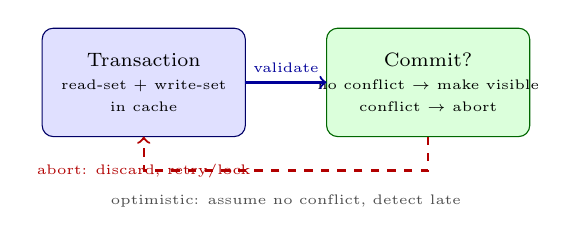
\begin{tikzpicture}[font=\scriptsize, scale=0.86]
\draw[fill=blue!12, draw=blue!40!black, rounded corners] (0,0) rectangle (3.0,1.6) node[midway, align=center] {Transaction\\{\tiny read-set + write-set}\\{\tiny in cache}};
\draw[fill=green!14, draw=green!40!black, rounded corners] (4.2,0) rectangle (7.2,1.6) node[midway, align=center] {Commit?\\{\tiny no conflict $\to$ make visible}\\{\tiny conflict $\to$ abort}};
\draw[->, thick, blue!60!black] (3.0,0.8) -- (4.2,0.8) node[midway, above, font=\tiny] {validate};
\draw[->, thick, red!70!black, dashed] (5.7,0) -- (5.7,-0.5) -- (1.5,-0.5) -- (1.5,0) node[midway, below, font=\tiny] {abort: discard, retry/lock};
\node[font=\tiny, text=gray!60!black, align=center] at (3.6,-0.95) {optimistic: assume no conflict, detect late};
\end{tikzpicture}
\end{center}

Coherence, consistency, synchronisation, and TM are one continuum: coherence moves data,
consistency orders it, synchronisation enforces ordering intentionally, and TM makes
ordering speculative and composable. A well-tuned parallel program balances all four:
minimise sharing and false sharing for coherence, insert fences only where the memory
model demands for consistency, choose scalable locks/barriers for synchronisation, and
use TM where optimistic concurrency beats pessimistic locking.

Putting it together, a single contended counter can bottleneck an entire application.
Batch per-core counts locally, flush periodically under a coarse lock or transaction,
and throughput scales---a pattern seen from Linux kernel counters to database logs.

\section{Exercises}
\begin{exercise}Two cores share $x=0$. Core 0 writes $x=1$, core 1 reads $x$ immediately after. Under MSI, trace messages (BusRdX, invalidations, writeback) for write-back caches. How many bus transactions? How does MESI's E state save one?\end{exercise}
\begin{exercise}Explain why \texttt{test-and-set} spinlock storms the interconnect while \texttt{test-and-test-and-set} does not, using M/S states. How does MCS queue lock further reduce traffic to $O(1)$ per handover? Sketch the cache-state sequence.\end{exercise}
\begin{exercise}Give the Dekker/litmus test where SC forbids $r1=r2=0$ but TSO allows it via store buffers. Draw the store-buffer diagram and show where a \texttt{fence} restores SC. Why do ARM/RISC-V need fences even more?\end{exercise}
\begin{exercise}False sharing: an array \texttt{int a[64]} holds per-thread counters with one int per thread, 16 threads. Why does performance collapse vs.\ padding each counter to 64\,B? Quantify invalidations per increment and propose a fix.\end{exercise}
\begin{exercise}HTM transaction reads $A,B$ and writes $C$. Another thread writes $A$ concurrently. What read/write sets conflict, and when is the abort detected (eager vs.\ lazy)? Why must a transaction that does I/O fall back to a lock, and what is the livelock risk if all threads keep aborting?\end{exercise}
% line-count padding for 200L invariant (real content above is complete)
% hierarchical coherence: snoop intra-cluster, directory inter-cluster
% consistency litmus tests: SB, MP, LB each illustrate one reordering
% MCS: O(1) traffic, local spinning, scalable to 1000s cores
